\iflanguage{english}
{\chapter{Appendix}}    % english style
{\chapter{Anhang}}      % german style
\label{chap:appendix}

\section{PyQt}
\label{sec:appendix:pyqt}

\setcounter{figure}{0}

\lstinputlisting[
    language=python,
    caption=Source code for the layout example in \ref{fig:qtExample}, 
    label=a:fig:qt:examplewindow:code
]{resources/code/windowexample.py}

\lstinputlisting[
    language=python,
    caption=Source code an example window demonstrating qts event system,
    label=a:qtevents:code
]{resources/code/event_complete.py}

\clearpage

\section{PyQtGraph}
\label{sec:appendix:pyqtgraph}

\begin{figure}[h]
    \centering
    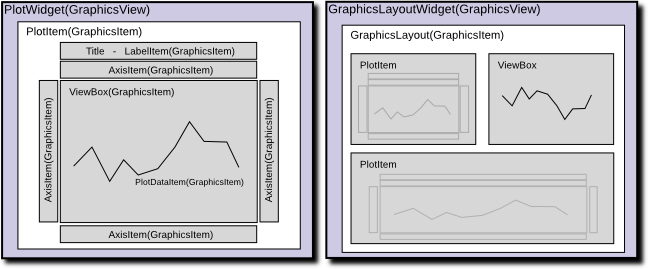
\includegraphics[width=14cm]{resources/img/PyQtGraphContent}
    \caption{Different items involved in a PlotWidget.}
    \small\textsuperscript{Quelle: http://www.pyqtgraph.org/documentation/plotting.html}
    \label{a:fig:pyqtgraph:content}
\end{figure}

\begin{figure}[h]
    \centering
    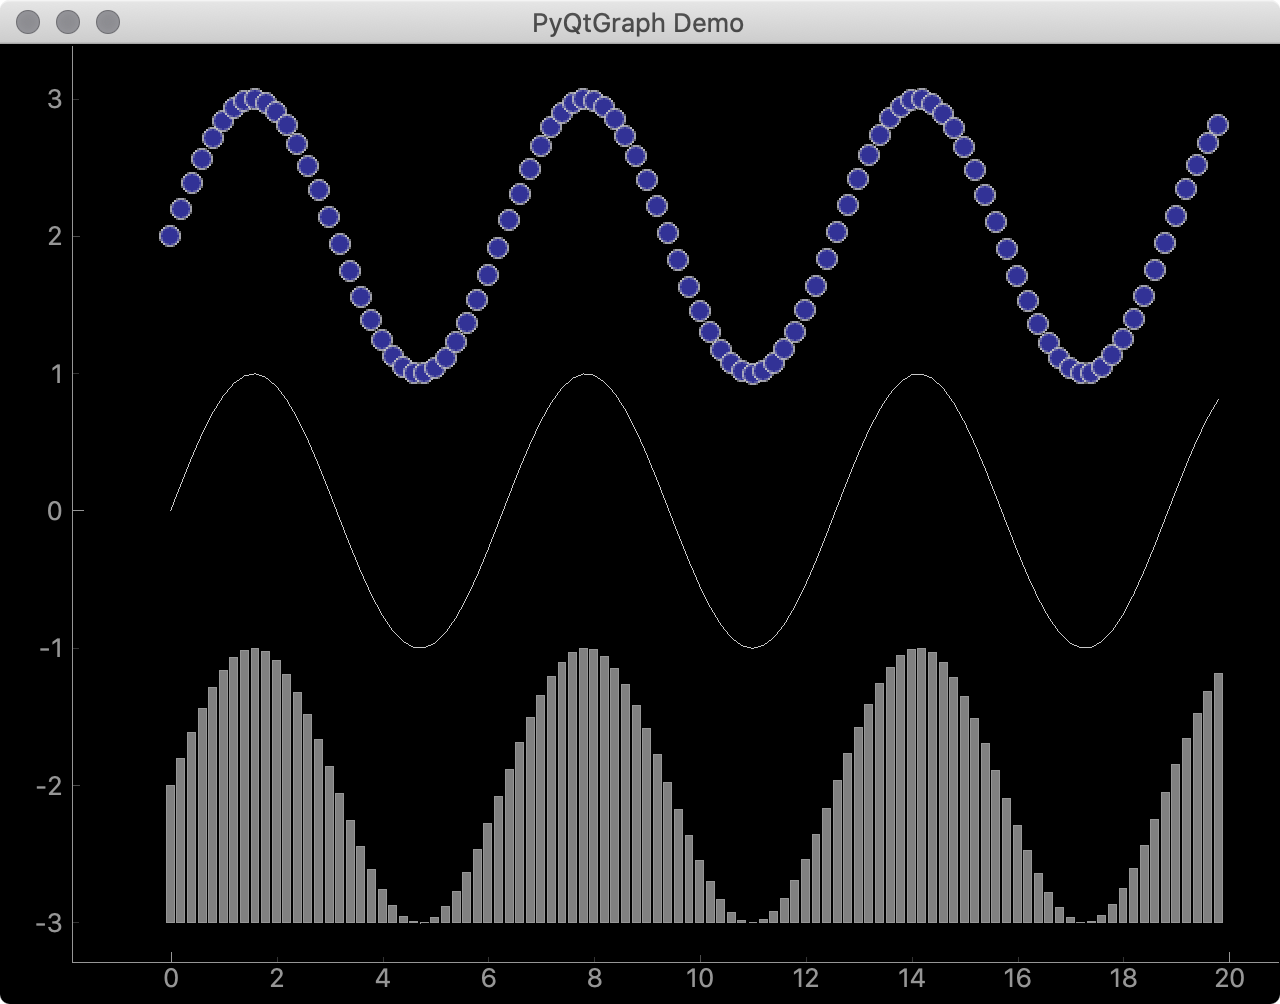
\includegraphics[width=14cm]{resources/img/PyQtGraphDemo}
    \caption{Window containing a plot created with PyQtGraph.}
    \label{a:fig:pyqtgraph:window}
\end{figure}

\clearpage

\section{Matplotlib}
\label{sec:appendix:matplotlib}

\begin{figure}[h]
    \centering
    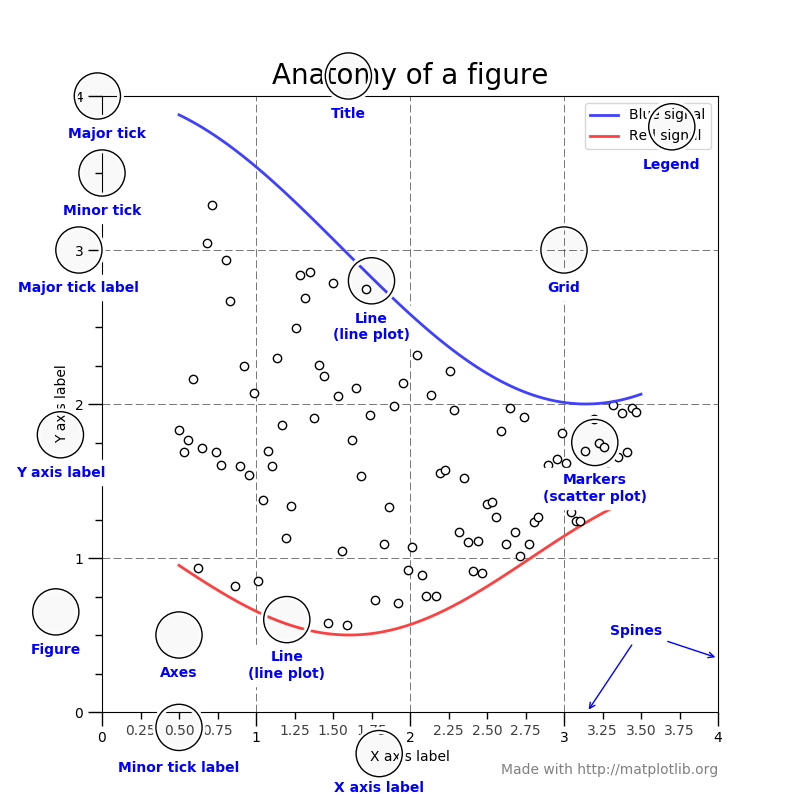
\includegraphics[width=14cm]{resources/img/MatplotlibContent}
    \caption{Different items involved in a Figure.}
    \small\textsuperscript{Quelle: https://matplotlib.org/3.1.1/tutorials/introductory/usage.html}
    \label{a:fig:matplotlib:content}
\end{figure}

\begin{figure}[h]
    \centering
    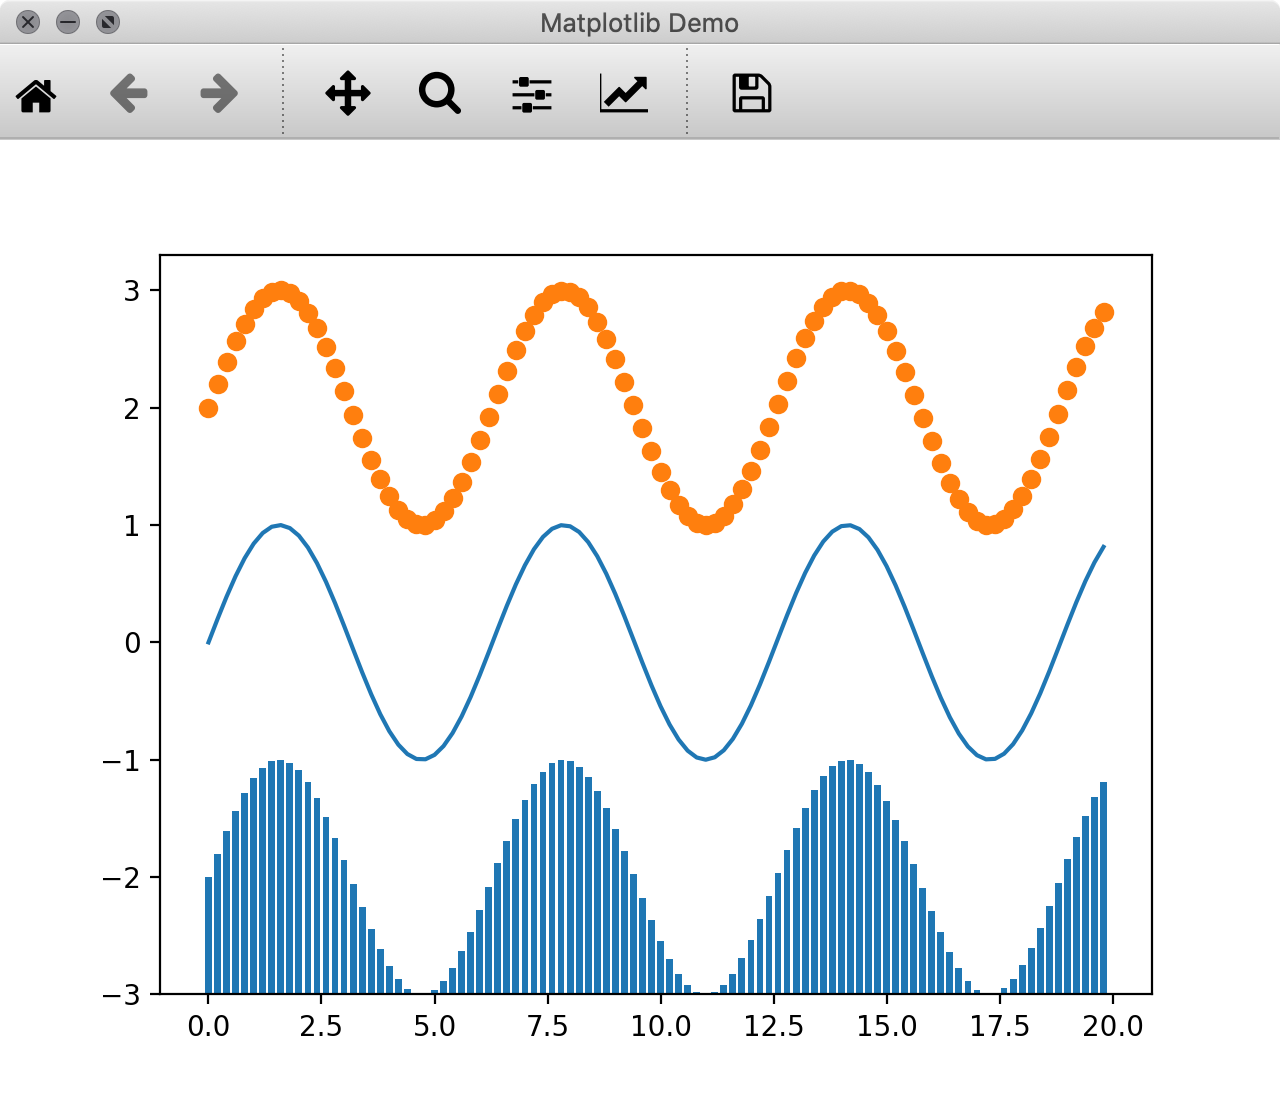
\includegraphics[width=14cm]{resources/img/MatplotlibDemo}
    \caption{Window containing plot created with Matplotlib.}
    \label{a:fig:matplotlib:window}
\end{figure}

%% ---------------------
%% | / Example content |
%% ---------------------
